\subsection{Processamento de imagem}

De forma complementar ao assunto supracitado, o processamento de imagem evoluiu drasticamente no decorrer do avanço tecnológico. Portanto, há grande interesse nessa tecnologia pelo fato de proporcionar um grande número de aplicações, como por exemplo o aprimoramento de informações relativo a imagens para interpretação humana e análise automáticas por computador de informações extraídas da imagem capturada.

Contudo, o grande marco da área de processamento de imagens aconteceu no século XX. Com o surgimento dos primeiros computadores digitais com grande capacidade de processamento e o início do programa espacial norte-americano, ocorreu um grande impulso na área de processamento de imagem. O uso de técnicas computacionais de aprimoramento de imagens teve início no \textit{Jet Propulsion Laboratory} (Laboratório de Propulsão a Jato), localizado no centro tecnológico da NASA, em 1964, quando "imagens da lua transmitidas por uma sonda Ranger eram processadas por computador para corrigir vários tipos de distorção inerentes à câmera de TV acoplada à sonda". Essa tecnologia foi usada em grandes expedições tripuladas, como a Apollo \cite{FILHO1999}.

Para realizar o processamento de uma imagem, são definidos passos a serem seguidos para a garantia do objetivo final. A captura da imagem consiste no uso de dispositivos físicos sensíveis a espectros de energia eletromagnética que convertem o sinal elétrico para um formato digital. O pré-processamento consiste no realce da imagem para enfatizar características de interesse ou recuperar imagens que sofreram alguma degradação devido à introdução de ruído, perda de contraste ou borramento. A segmentação é a extração ou identificação dos objetos contidos na imagem, separando a imagem em regiões. Por fim, a classificação, é o processo que identifica a imagem observada \cite{GONZALEZ2002}.

As etapas básicas do processamento de imagem estão representadas através da \autoref{fig_etapas-processamento-imagem}.

\begin{figure}[h]
	\caption{\label{fig_etapas-processamento-imagem}Etapas básicas do processamento de imagens.}
	\begin{center}
		
\includegraphics[scale=0.5]{4-Conteudo-Bibliografico/2-Visao-Computacional/Imagens-Visao-Computacional/etapas-processamento-imagem.jpg}
	\end{center}
	\centering \legend{Fonte: Adaptada de \citeonline{GONZALEZ2002}}
\end{figure}

Seres humanos conseguem distinguir vários padrões de cores com certa facilidade, levando em consideração que a análise é feita em um ambiente tridimensional. Na computação, esse discernimento de cores são mais complexos, independentemente da dimensão na qual a imagem será analisada. Isso ocorre porque vários fatores podem contribuir para a má performance computacional no tratamento da imagem, como por exemplo a falta ou excesso de luz, qualidade do sensor, qualidade da imagem, dentre outros.

\begin{quotation}
“Objetos que emitem luz visível são percebidos em função da soma das cores espectrais emitidas. Tal processo de formação é denominado aditivo. O processo aditivo pode ser interpretado como uma combinação variável em proporção de componentes monocromáticas nas faixas espectrais associadas às sensações de cor verde, vermelho e azul, as quais são responsáveis pela formação de todas as demais sensações de cores registradas pelo olho humano. Assim, as cores verde, vermelho e azul são ditas cores primárias. Este processo de geração suscitou a concepção de um modelo cromático denominado RGB (Red, Green, e Blue), para o qual a Comissão Internacional de Iluminação (CIE) estabeleceu as faixas de comprimento de onda das cores primárias.” \cite{QUEIROZ2006}
\end{quotation}

Cada \textit{pixel} é representado por um valor numérico que corresponde a sua cor em questão. Sendo assim, para que seja possível representar uma imagem em alguma escala de cor monocromática (preto e branco, ou escalas de cinza), basta associar o \textit{pixel} a um valor numérico relacionado a sua escala de tom.

A \autoref{fig_rep-pixel-monocromatico} exemplifica a associação dos \textit{pixels} de forma a obter uma imagem monocromática. Segundo \citeonline{NELMA2000}, para obter uma imagem em tons de cinzento, basta associar cada \textit{pixel} um valor inteiro não negativo de um byte, onde o valor 0 corresponde a cor preta e o valor máximo, 255, corresponde a cor branca. Os valores intermediários correspondem aos variados tons de cinza.

\begin{figure}[h]
	\caption{\label{fig_rep-pixel-monocromatico}Visão computacional de \textit{pixel} monocromático.}
	\begin{center}
		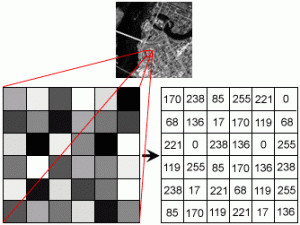
\includegraphics[scale=3.5]{4-Conteudo-Bibliografico/2-Visao-Computacional/Imagens-Visao-Computacional/rep-pixel-monocromatico.jpg}
	\end{center}
	\centering \legend{Disponível em: https://ai.stanford.edu/~syyeung/cvweb/tutorial1.html}
\end{figure}

Já as imagens coloridas exigem um poder maior de processamento para serem reconhecidas. Isso ocorre porque as imagens em RGB - \textit{Red, Green, and Blue} (Vermelho, Verde e Azul)  precisam de mais de uma banda para serem processadas, ou seja, são analisadas três matrizes de cores para formar a paleta de cor específica do tom capturado (\autoref{fig_rgb-representacao}). Depois da análise, são formadas as cores distintas que compõe a imagem.

\begin{figure}[h]
	\caption{\label{fig_rgb-representacao}Matriz de \textit{pixels} RGB.}
	\begin{center}
		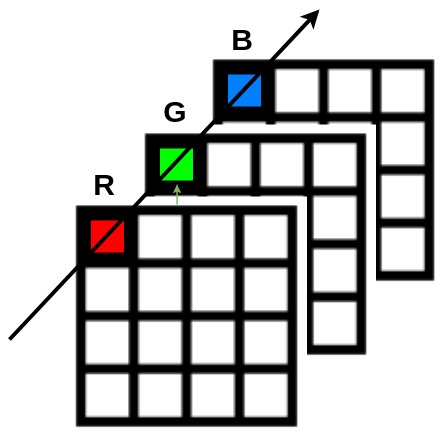
\includegraphics[scale=0.3]{4-Conteudo-Bibliografico/2-Visao-Computacional/Imagens-Visao-Computacional/rgb-representacao.jpg}
	\end{center}
	\centering \legend{Fonte: Elaborada pelos autores do projeto.}
\end{figure}

De forma mais detalhada, \citeonline{LOPES2013} exemplificam que imagens coloridas também são imagens multibanda, ou multiespectral. As cores visíveis através de olhos humanos podem ser representadas pela combinação de bandas das cores primárias vermelha, verde e azul (\textit{Red, green} e \textit{blue}, respectivamente). A imagem colorida também pode ser armazenada por meio de imagens cromáticas e mapas de cores. Nesse caso, o valor de cinza de cada \textit{pixel} na imagem se torna um índice para uma entrada de mapa de cores, enquanto a entrada em si do mapa de cores contem os valores dos componentes referentes as tonalidades \textit{RGB} (\autoref{fig_rep-pixel-rgb}).

\begin{figure}[h]
	\caption{\label{fig_rep-pixel-rgb}Visão computacional de \textit{pixels} RGB.}
	\begin{center}
		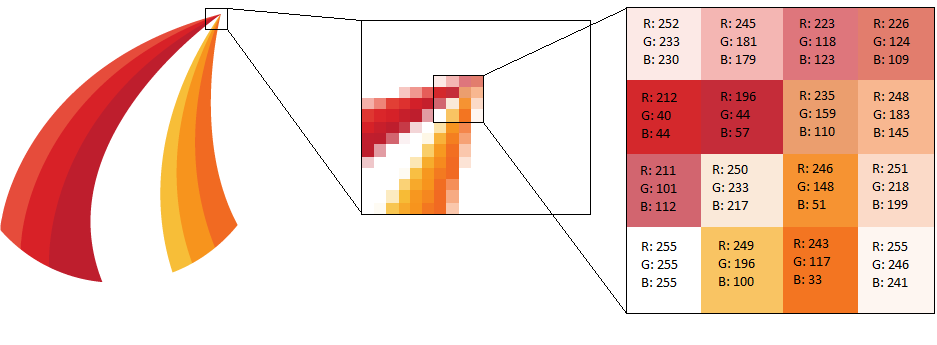
\includegraphics[scale=0.4]{4-Conteudo-Bibliografico/2-Visao-Computacional/Imagens-Visao-Computacional/rep-pixel-rgb.png}
	\end{center}
	\centering \legend{Disponível em: https://www.analyticsindiamag.com/computer-vision-primer-how-ai-sees-an-image/}
\end{figure}

No entanto, a imagem capturada por algum dispositivo eletrônico pode chegar de forma irregular ate a parte de processamento. Essas falhas podem ser caracterizadas de várias formas, como por exemplo a presença de \textit{pixels} ruidosos, brilho e/ou contrastes desregulados, caracteres com dígitos incompletos ou apagados como em digitalizações de documentos.

A parte de processamento fica responsável por elaborar uma melhoria da imagem em questão, ajustando todos os parâmetros para que seja possível analisar precisamente todas as informações que estão disponíveis no arquivo de imagem. Sendo assim, por analogia as imagens processadas, trata-se de uma etapa que analisa de forma profunda todos os dados contidos na imagem, ou seja, a fase de processamento abrange os níveis mais baixos de análise de imagens, pois trabalham diretamente com valores de intensidade dos \textit{pixels}, visto que neste período não existe nenhuma informação relacionada a imagem para que seja possível facilitar o trabalho. O resultado desse processo gera imagens digitalizadas de qualidade melhor que a original.